\chapter{Comparaci\'on con otras alternativas}\label{alternativas}

\section{Competidores considerados}

Para el an\'alisis competitivo se han considerado cinco soluciones de referencia en el
mercado espa\~nol de comparaci\'on de compra:

\begin{itemize}
	\item Soysuper
	\item Findit
	\item OCU Market
	\item PreciRadar
	\item RadarPrice
\end{itemize}

Adicionalmente, se han valorado como competencia indirecta las apps nativas de cadenas
y como sustituto no tecnol\'ogico la comparaci\'on manual con folletos.

\section{Matriz funcional resumida}

\begin{table}[htbp]
\centering
\caption{Comparativa de capacidades clave}
\label{tab:comparativa-alternativas}
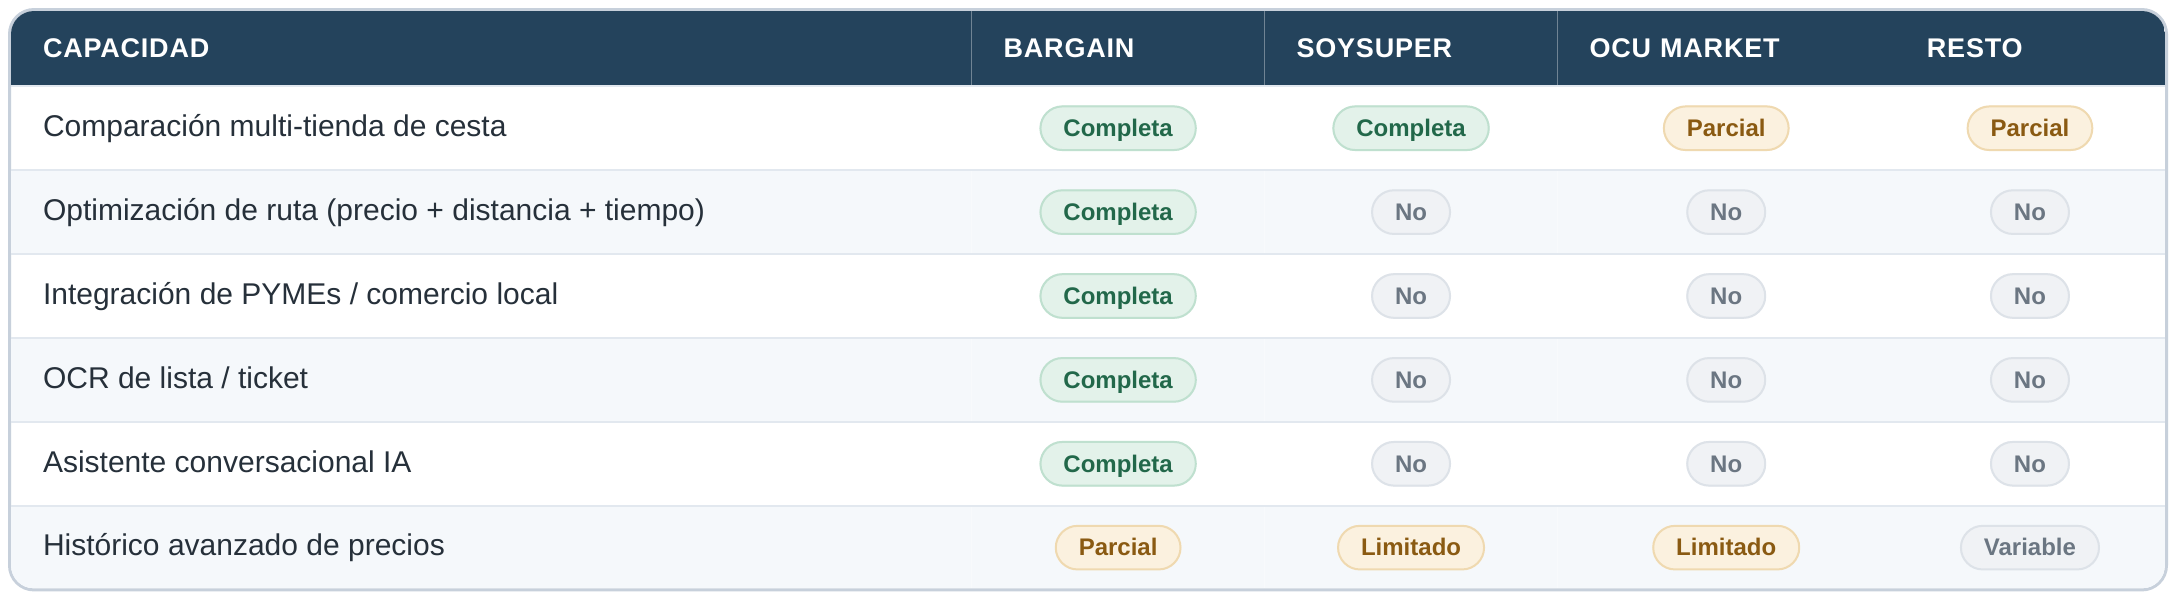
\includegraphics[width=0.95\textwidth]{diagramas/cuadros/cuadro-comparativa-alternativas.png}
\end{table}

\section{Brechas estrat\'egicas detectadas}

El an\'alisis identifica cuatro brechas de mercado que justifican la propuesta:

\begin{enumerate}
	\item \textbf{Gap precio-ruta:} los comparadores muestran precios, pero no optimizan
		desplazamiento y tiempo.
	\item \textbf{Comercio local invisible:} no existe cobertura estable de PYMEs en
		herramientas generalistas.
	\item \textbf{Fricci\'on de entrada:} la lista de compra sigue siendo manual en la mayor\'ia
		de soluciones.
	\item \textbf{Interacci\'on limitada:} predominan filtros y b\'usquedas r\'igidas frente a
		consultas en lenguaje natural.
\end{enumerate}

\section{Posicionamiento de BargAIn}

BargAIn se posiciona como un \emph{optimizador inteligente de compra} y no solo como
comparador. Su propuesta de valor combina ahorro econ\'omico, eficiencia log\'istica y
experiencia de usuario asistida por IA.

\section{Riesgos competitivos}

Los riesgos principales identificados son:

\begin{itemize}
	\item reacci\'on de competidores consolidados con mayor base de usuarios,
	\item dependencia de fuentes de datos de terceros para scraping,
	\item necesidad de mantener alta calidad de datos para sostener confianza.
\end{itemize}

Como mitigaci\'on, se adopta una estrategia de fuentes h\'ibridas de datos, modularidad
arquitect\'onica y pipeline de validaci\'on continua.
